% Standalone source of the common-theta bundle sketch used in Sec. 3.6 of the paper.
% Compile: pdflatex fig_bundle.tex   (produces fig_bundle.pdf, included by paper.tex)
\documentclass[border=8pt]{standalone}
\usepackage{tikz}
\usepackage{amsmath,amssymb}
\begin{document}
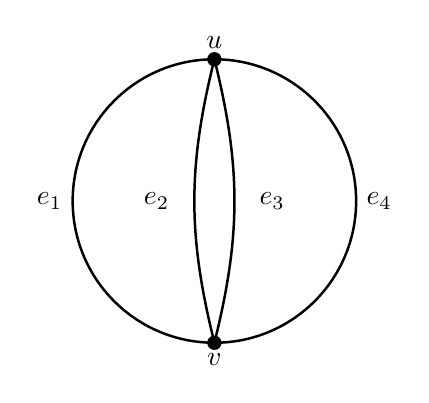
\begin{tikzpicture}[line width=0.9pt]
  % The two vertices of the bundle; neither carries an external line.
  \coordinate (U) at (0,1.8);
  \coordinate (V) at (0,-1.8);
  % Outer two lines: the left and right halves of one circle.
  \draw (U) arc (90:270:1.8);
  \draw (U) arc (90:-90:1.8);
  % Inner two lines: near-vertical chords joining the same pair of vertices.
  \draw (U) to[bend right=14] (V);
  \draw (U) to[bend left=14] (V);
  % Vertices.
  \fill (U) circle (2.6pt);
  \fill (V) circle (2.6pt);
  \node[above] at (U) {$u$};
  \node[below] at (V) {$v$};
  % Line labels.
  \node[left] at (-1.8,0) {$e_1$};
  \node[left] at (-0.44,0) {$e_2$};
  \node[right] at (0.44,0) {$e_3$};
  \node[right] at (1.8,0) {$e_4$};
\end{tikzpicture}
\end{document}
